\section{Backend Unit Test}
For the Backend JUnit and Maven were used to set up the Unit Tests. In these Unit Tests the goal was to detect whether there were any failures or errors regarding any subsection of the project.
Tests were conducted on each module to determine the results.

\subsection{Dependencies required}
To set up the tests we had to add dependencies to the pom.xml file. These dependencies made use of JUnit to create and test all unit tests.
JUnit is a simple framework to write repeatable tests.
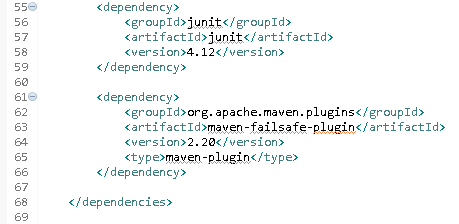
\includegraphics[]{backend/data/Dependencies_needed.png}

\subsection{Setting up Unit Test}
To create the unit test, a standard Java class is created. Inside this class an instance of the module to be tested was instantiated and annotated with JUnit annotations.
Then each property of the object was asserted and its validity tested.
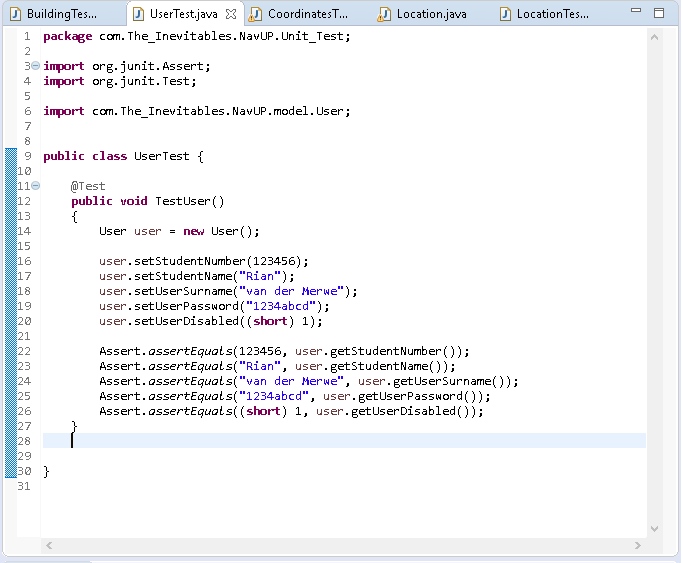
\includegraphics[]{backend/data/User_Unit_Test.png}

\subsection{Running Unit Test}
To execute the unit tests the following command is executed: mvn test. This will compile the project and test all classess annotated as @Test classes.

\subsection{Results}
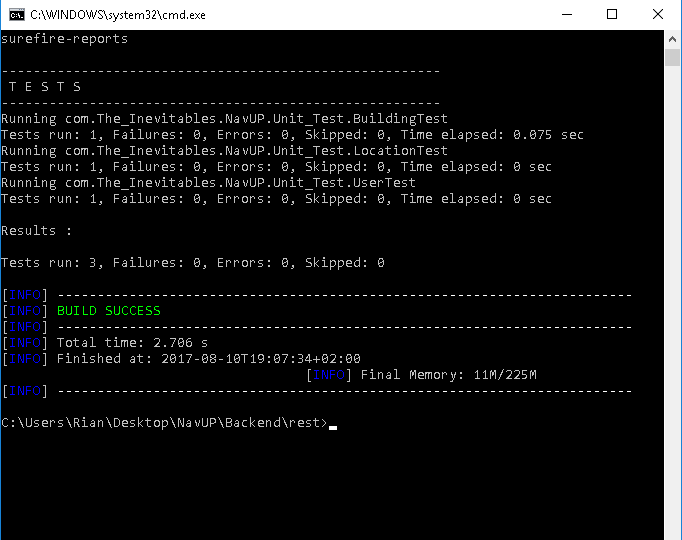
\includegraphics[]{backend/data/Backend_Unit_Tests.png}
